\section{Objekterkennung}
\begin{frame}
    \frametitle{Bedingungen durch das Carolo-Cup Regelwerk
    \footnote{Grafiken basierend auf: \xfootcite{Carolo-CupRegelwerk}}}
    \begin{columns}
        \begin{column}{.33\textwidth}
            \includegraphics[height=.45\textheight]{../Material/Presentation/Obstacle.pdf}
        \end{column}
        \pause
        \begin{column}{.33\textwidth}
            \includegraphics[height=.45\textheight]{../Material/Presentation/Pedestrian.pdf}
        \end{column}
        \pause
        \begin{column}{.33\textwidth}
            
\includegraphics[height=.45\textheight]{../Material/Presentation/Sign.pdf}
        \end{column}
    \end{columns}
    \pause
    \begin{itemize}
        \item Hindernisse und Fußgänger sind nicht anhand der Punktwolke unterscheidbar
            \pause
        \item Steigungen mit bis zu $10^\circ$
    \end{itemize}
\end{frame}

\begin{frame}
    \frametitle{Stand der Technik}
    \begin{itemize}
        \item Kombinierte Detektion und Klassifikation mit \acf{cnn}
            \pnote{Punktwolke oftmals als Voxel oder 2D-Karte repräsentiert}
            \pause
        \item Langsam ohne \ac{gpu} (Abschätzung: $30\si{\s}$ für Complex-YOLO)
            \pnote{Abschätzung auf Basis von YOLO auf Fahrzeug}
            \pause
        \item Schneller: Seperate Detektion und Klassifikation
            \pnote{Clustering mit ConnComp, Klassifikation mit K-NN, SVM, CNN}
            \pause
        \item Primär für Lidar Daten
            \pnote{Stereo PWs sind dichter aber mehr outlier}
            \pause
        \item Für Stereo: Oftmals auf Disparitätsbildern
            \pnote{Nachbarschaft nicht korrekt}
            \pause
        \item Nachbarschaft wird in Punktwolken besser repräsentiert \xfootcite{Wang19}
            \pnote{Standard Lidar Algorithmen auf Stereo PWs besser als SOTA für Disparitätsbilder}
    \end{itemize}
\end{frame}

\begin{frame}
    \frametitle{Algorithmus}
    \begin{itemize}
        \item Adaptierte Version von \cite{AttBen17}\xfootcite{AttBen17} für Stereodaten
            \pnote{Getrennte Pipeline, anpassungen für Stereo}
            \pause
        \item Vorgehen: 
            \pause
            \begin{itemize}
                \item Segmentierung
                    \pnote{Jedem Punkt eine Klasse zuordenen}
                    \pause
                \item Clustering
                    \pnote{Punkte gleicher Klasse zusammenfassen}
                    \pause
                \item Extraktion von Pseudotiefenbilder
                    \pnote{Klassifikation einfacher und schneller als auch PW}
                    \pause
                \item Klassifikation
                    \pnote{CNN}
                    \pause
            \end{itemize}
        \item Zusätzlich: Bounding-Box- und Bodenschätzung
            \pnote{Für spätere Plannung relevant}
    \end{itemize}
\end{frame}

\begin{frame}
    \frametitle{Algorithmus - Segmentierung}
    Klassen: Sparse, Ground, High-Foreground, Low-Foreground
    \begin{figure}
        \centering
        \includegraphics[width=\textwidth]{../Material/Presentation/grid.png}
    \end{figure}
    \pnote{Punktwolke in Zellen einordnen}
    \pnote{Wenn weniger als 8 Punkte dann Sparse}
    \pnote{Wenn Differenz Max-Min kleiner 0.25m dann Ground}
    \pnote{Wenn maximum 1.4m höher als Fahrzeug oder max-min > 3.1m dann HF}
    \pnote{Sonst LF}
\end{frame}

\begin{frame}
    \frametitle{Algorithmus - Clustering}
    \begin{figure}
        \centering
        \includegraphics[width=\textwidth]{../Material/Presentation/objects.png}
    \end{figure}
    \pnote{Connecte Components auf zwei Ebenen}
    \pnote{Zuerst auf Zellen Ebene, mergen wenn Maximum-Differenz klein}
    \pnote{Dann jede Zelle in drei Subzellen teilen}
    \pnote{Cluster trennen wenn zu geringe Dichtedifferenz zwischen Subzellen}
\end{frame}

\begin{frame}
    \frametitle{Ausrichtung bestimmen}
    \begin{columns}
        \begin{column}{.5\textwidth}
            \begin{itemize}
                \item<1-> Hauptkomponenten-analyse des Clusters
                    \pnote{Richtungen mit größter Veränderung finden}
                \item<2-> Wichtigste nicht vertikale Hauptachse
                    \pnote{Für hohe Objekte, z.B. Fußgänger, ist erste HA quasi Vertikal}
                \item<3-> Für erste HA: Winkel zur $z$-Achse bestimmen
                    \pnote{Dadurch feststellen ob primär horizontal oder vertikal}
                \item<4-> Wenn größer als $45^\circ$ dann erste Hauptachse
                    \pnote{Entsprechende horizontale Komponente der HA nehmen}
            \end{itemize}
        \end{column}
        \begin{column}{.5\textwidth}
            \begin{figure}
                \centering
                \begin{tikzpicture}
                    \node[anchor=south west,inner sep=0] at (0,0) {
                        \includegraphics[width=\textwidth]{pca.png}
                    };
                    \coordinate (0) at (2.42,2.37);
                    \coordinate (y) at (2.27,4.43);
                    \coordinate (b) at (2.4,4.47);
                    \coordinate (g) at (4.52,2.0);
                    \coordinate (x) at (4.52,2.07);
                    
                    \draw[white,line width=0.6mm,->] (0) -- (y);
                    \draw[white,line width=0.6mm,->] (0) -- (x);
                    \draw[green,line width=0.6mm,->] (0) -- (g);
                    \draw[blue, line width=0.6mm,->] (0) -- (b);
                \end{tikzpicture}
            \end{figure}
        \end{column}
    \end{columns}
\end{frame}

\begin{frame}
    \frametitle{Algorithmus - Extraktion und Klassifikation}
    \pnote{Projektionsebene aus Heading und z-Achse}
    \pnote{Alle Punkte aus Projektionsebene projezieren, Helligkeit je nach Entfernung}
    \pnote{Größe 96x96}
    \begin{columns}
        \begin{column}{.5\textwidth}
            \begin{figure}
                \centering
                \includegraphics[width=\textwidth]{../Material/Presentation/image_0.png}
                \caption{Hindernis}
            \end{figure}
        \end{column}
        \begin{column}{.5\textwidth}
            \begin{figure}
                \centering
                \includegraphics[width=\textwidth]{../Material/Presentation/image_2.png}
                \caption{Schild}
            \end{figure}
        \end{column}
    \end{columns}
    \pause
    Klassifikation mit \ac{cnn}: Vehicle, Short Facade, Street Clutter, Pedestrian
    \pnote{4 Conv, Dense, Softmax}
\end{frame}

\begin{frame}
    \frametitle{Verbesserungen - Segmentierung}
    \begin{itemize}
        \item Low- und High-Foreground kombiniert
            \pnote{Carolo-Cup kennt nur kleine Objekte, Unterscheidung nicht relevant}
            \pause
        \item Klassifikation über minimum/maximum anfällig
            \pnote{Stereo PWs haben viele Outlier, minimum und maximum wird nur durch einen Punkt bestimmt}
            \pause
        \item Klassifikation über Varianz
            \pnote{Varianz robuster, beschreibt auch die Höhenverteilung}
    \end{itemize}
\end{frame}

\begin{frame}
    \frametitle{Verbesserungen - Extraktion und Klassifikation}
    \begin{itemize}
        \item Hauptkomponentenanalyse nicht notwendig
            \pnote{Boxen unabhängig von Betrachtungsrichtung}
            \pnote{Schilder am meisten Informationen von vorne}
            \pause
        \item Kleinere Pseudotiefenbilder
            \pnote{Alle Informationen in 40x40 Pixel}
            \pause
        \item Median-Filter für Distanzinvarianz
            \pnote{Um Löcher zu schließen}
            \pause
        \item Nur drei Klassen: Obstacle, Clutter, Pedestrian
            \pnote{Gibt keine Short Facade laut Regelwerk}
            \pause
        \item Kleineres \ac{cnn} ausreichend
            \pnote{Schneller, Input Kleiner, nur 2 Conv}
            \pause
        \item Trainingsdatensatz: 2406 Bilder
            \pnote{Training mit Data-Augmentation x10, Max-Pooling, Adadelta}
    \end{itemize}
\end{frame}

\begin{frame}
    \frametitle{Verbesserungen - Textur}
    \begin{itemize}
        \item Für Kitti/Lehr: Farbinformation für jeden Punkt
            \pnote{Da direkt von Farbkamera kommen information direkt vorhanden}
            \pause
        \item Wird statt Tiefeninformation genutzt
            \pnote{Dadurch komplexe Objekte gut zu unterscheiden}
            \pause
    \end{itemize}
    \begin{figure}[h!]
        \centering
        \begin{subfigure}[c]{0.3\textwidth}
            \includegraphics[width=\textwidth]{../Material/texture222_0.png}
        \end{subfigure}
        \begin{subfigure}[c]{0.3\textwidth}
            \includegraphics[width=\textwidth]{../Material/texture222_1.png}
        \end{subfigure}
        \begin{subfigure}[c]{0.3\textwidth}
            \includegraphics[width=\textwidth]{../Material/texture0_0.png}
        \end{subfigure}
    \end{figure}
\end{frame}

\begin{frame}
    \frametitle{Erweiterungen - Bounding Box}
    \begin{columns}
        \begin{column}{.5\textwidth}
            \begin{itemize}
                \item Zum Umfahren von Hindernissen/Fußgängern, bzw. Klassifikation von Schilder 
                    \pnote{In beiden Fällen ist groß nicht schlecht}
                \item<2-> Zuerst Ausrichtung bestimmen
                    \pnote{Verweis auf Hauptkomponentenanalyse}
                \item<3-> Dann Ausdehnung in $x$ und $y$ Richtung bestimmen
                    \pnote{Entlang der Hauptachse, z Ignorieren}
                \item<4-> Ausdehnung in $z$ Richtung bestimmen
                    \pnote{Hier keine Drehung, da alles flach}
            \end{itemize}
        \end{column}
        \begin{column}{.5\textwidth}
            \only<1>{
    \begin{figure}[h!]
        \centering
        \begin{tikzpicture}
            \fill[fill=primary] (4,4) circle (0.2cm);
            \fill[fill=primary] (4.5,4.5) circle (0.2cm);
            \fill[fill=primary] (5,5) circle (0.2cm);
            \fill[fill=primary] (5.5,5.5) circle (0.2cm);
            \fill[fill=primary] (6,6) circle (0.2cm);
            \fill[fill=primary] (4.5,5.5) circle (0.2cm);
            \fill[fill=primary] (5.5,4.5) circle (0.2cm);
            \fill[fill=primary] (4,5) circle (0.2cm);
            \fill[fill=primary] (6,5) circle (0.2cm);
            \fill[fill=primary] (5,4) circle (0.2cm);
            \fill[fill=primary] (5,6) circle (0.2cm);

            \node at(3,3) (){};
            \node at(7.5,7.5) (){};
        \end{tikzpicture}
    \end{figure}
}
\only<2>{
    \begin{figure}[h!]
        \centering
        \begin{tikzpicture}
            \fill[fill=primary] (4,4) circle (0.2cm);
            \fill[fill=primary] (4.5,4.5) circle (0.2cm);
            \fill[fill=primary] (5,5) circle (0.2cm);
            \fill[fill=primary] (5.5,5.5) circle (0.2cm);
            \fill[fill=primary] (6,6) circle (0.2cm);
            \fill[fill=primary] (4.5,5.5) circle (0.2cm);
            \fill[fill=primary] (5.5,4.5) circle (0.2cm);
            \fill[fill=primary] (4,5) circle (0.2cm);
            \fill[fill=primary] (6,5) circle (0.2cm);
            \fill[fill=primary] (5,4) circle (0.2cm);
            \fill[fill=primary] (5,6) circle (0.2cm);

            \draw[line width=2pt,->] (5,5) -- (7,7);

            \node at(3,3) (){};
            \node at(7.5,7.5) (){};
        \end{tikzpicture}
    \end{figure}
}
\only<3->{
    \begin{figure}[h!]
        \centering
        \begin{tikzpicture}
            \fill[fill=primary] (4,4) circle (0.2cm);
            \fill[fill=primary] (4.5,4.5) circle (0.2cm);
            \fill[fill=primary] (5,5) circle (0.2cm);
            \fill[fill=primary] (5.5,5.5) circle (0.2cm);
            \fill[fill=primary] (6,6) circle (0.2cm);
            \fill[fill=primary] (4.5,5.5) circle (0.2cm);
            \fill[fill=primary] (5.5,4.5) circle (0.2cm);
            \fill[fill=primary] (4,5) circle (0.2cm);
            \fill[fill=primary] (6,5) circle (0.2cm);
            \fill[fill=primary] (5,4) circle (0.2cm);
            \fill[fill=primary] (5,6) circle (0.2cm);

            \draw[line width=2pt,->] (5,5) -- (7,7);
            \coordinate (a) at (4.5, 3.2);
            \coordinate (b) at (6.8, 5.5);
            \coordinate (c) at (5.5, 6.8);
            \coordinate (d) at (3.2, 4.5);
            \draw[line width=2pt] (a) -- (b);
            \draw[line width=2pt] (b) -- (c);
            \draw[line width=2pt] (c) -- (d);
            \draw[line width=2pt] (d) -- (a);

            \node at(3,3) (){};
            \node at(7.5,7.5) (){};
        \end{tikzpicture}
    \end{figure}
}

        \end{column}
    \end{columns}
\end{frame}

\begin{frame}
    \frametitle{Erweiterungen - Bodenschätzung}
    \begin{columns}
        \begin{column}{.5\textwidth}
            \begin{itemize}
                \item Alle Ground-Zellen werden Berücksichtigt
                    \pnote{Verweis Segmentierung}
                \item<2-> Mittel der $z$-Werte pro Zelle
                    \pnote{Mittlere Höhe in Zelle}
                \item<3-> Pro Zelle ein Punkt
                    \pnote{In mitte der Zelle mit Mittelwert $z$ als Höhe}
                \item<4-> Ebene mit Methode der kleinsten Quadrate
                    \pnote{Nur eine Ebene, am Anfang von Steigungen kann problematisch}
            \end{itemize}
        \end{column}
        \begin{column}{.5\textwidth}
            \only<1>{
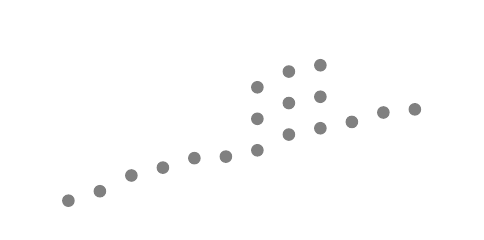
\begin{tikzpicture}[scale=0.4]
    \fill[fill=gray] (0,-0.2) circle (0.2cm);
    \fill[fill=gray] (1,0.1) circle (0.2cm);
    \fill[fill=gray] (2,0.6) circle (0.2cm);
    \fill[fill=gray] (3,0.85) circle (0.2cm);
    \fill[fill=gray] (4,1.15) circle (0.2cm);
    \fill[fill=gray] (5,1.2) circle (0.2cm);
    \fill[fill=gray] (6,1.4) circle (0.2cm);
    \fill[fill=gray] (7,1.9) circle (0.2cm);
    \fill[fill=gray] (8,2.1) circle (0.2cm);
    \fill[fill=gray] (9,2.3) circle (0.2cm);
    \fill[fill=gray] (10,2.6) circle (0.2cm);
    \fill[fill=gray] (11,2.7) circle (0.2cm);

    \fill[fill=gray] (6,2.4) circle (0.2cm);
    \fill[fill=gray] (7,2.9) circle (0.2cm);
    \fill[fill=gray] (8,3.1) circle (0.2cm);
    \fill[fill=gray] (6,3.4) circle (0.2cm);
    \fill[fill=gray] (7,3.9) circle (0.2cm);
    \fill[fill=gray] (8,4.1) circle (0.2cm);

    \node at(-1,-0.25) (){};
    \node at(12,5) (){};
\end{tikzpicture}
}
\only<2>{
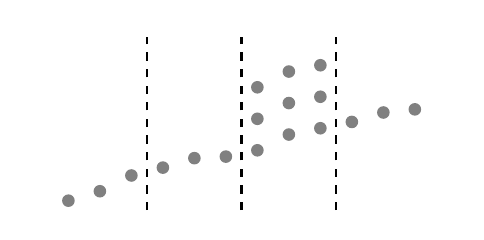
\begin{tikzpicture}[scale=0.4]
    \fill[fill=gray] (0,-0.2) circle (0.2cm);
    \fill[fill=gray] (1,0.1) circle (0.2cm);
    \fill[fill=gray] (2,0.6) circle (0.2cm);
    \fill[fill=gray] (3,0.85) circle (0.2cm);
    \fill[fill=gray] (4,1.15) circle (0.2cm);
    \fill[fill=gray] (5,1.2) circle (0.2cm);
    \fill[fill=gray] (6,1.4) circle (0.2cm);
    \fill[fill=gray] (7,1.9) circle (0.2cm);
    \fill[fill=gray] (8,2.1) circle (0.2cm);
    \fill[fill=gray] (9,2.3) circle (0.2cm);
    \fill[fill=gray] (10,2.6) circle (0.2cm);
    \fill[fill=gray] (11,2.7) circle (0.2cm);

    \fill[fill=gray] (6,2.4) circle (0.2cm);
    \fill[fill=gray] (7,2.9) circle (0.2cm);
    \fill[fill=gray] (8,3.1) circle (0.2cm);
    \fill[fill=gray] (6,3.4) circle (0.2cm);
    \fill[fill=gray] (7,3.9) circle (0.2cm);
    \fill[fill=gray] (8,4.1) circle (0.2cm);

    \draw[dashed, line width=0.3mm] (2.5,-0.5) -- (2.5,5);
    \draw[dashed, line width=0.3mm] (5.5,-0.5) -- (5.5,5);
    \draw[dashed, line width=0.3mm] (8.5,-0.5) -- (8.5,5);

    \node at(-1,-0.25) (){};
    \node at(12,5) (){};
\end{tikzpicture}
}
\only<3>{
\begin{tikzpicture}[scale=0.4]
    \fill[fill=gray] (0,-0.2) circle (0.2cm);
    \fill[fill=gray] (1,0.1) circle (0.2cm);
    \fill[fill=gray] (2,0.6) circle (0.2cm);
    \fill[fill=gray] (3,0.85) circle (0.2cm);
    \fill[fill=gray] (4,1.15) circle (0.2cm);
    \fill[fill=gray] (5,1.2) circle (0.2cm);
    \fill[fill=gray] (6,1.4) circle (0.2cm);
    \fill[fill=gray] (7,1.9) circle (0.2cm);
    \fill[fill=gray] (8,2.1) circle (0.2cm);
    \fill[fill=gray] (9,2.3) circle (0.2cm);
    \fill[fill=gray] (10,2.6) circle (0.2cm);
    \fill[fill=gray] (11,2.7) circle (0.2cm);

    \fill[fill=gray] (6,2.4) circle (0.2cm);
    \fill[fill=gray] (7,2.9) circle (0.2cm);
    \fill[fill=gray] (8,3.1) circle (0.2cm);
    \fill[fill=gray] (6,3.4) circle (0.2cm);
    \fill[fill=gray] (7,3.9) circle (0.2cm);
    \fill[fill=gray] (8,4.1) circle (0.2cm);

    \draw[dashed, line width=0.3mm] (2.5,-0.5) -- (2.5,5);
    \draw[dashed, line width=0.3mm] (5.5,-0.5) -- (5.5,5);
    \draw[dashed, line width=0.3mm] (8.5,-0.5) -- (8.5,5);

    \fill[fill=primary] (1,0.17) circle (0.2cm);
    \fill[fill=primary] (4,1.07) circle (0.2cm);
    \fill[fill=primary] (10,2.5) circle (0.2cm);

    \node at(-1,-0.25) (){};
    \node at(12,5) (){};
\end{tikzpicture}
}
\only<4>{
\begin{tikzpicture}[scale=0.4]
    \fill[fill=gray] (0,-0.2) circle (0.2cm);
    \fill[fill=gray] (1,0.1) circle (0.2cm);
    \fill[fill=gray] (2,0.6) circle (0.2cm);
    \fill[fill=gray] (3,0.85) circle (0.2cm);
    \fill[fill=gray] (4,1.15) circle (0.2cm);
    \fill[fill=gray] (5,1.2) circle (0.2cm);
    \fill[fill=gray] (6,1.4) circle (0.2cm);
    \fill[fill=gray] (7,1.9) circle (0.2cm);
    \fill[fill=gray] (8,2.1) circle (0.2cm);
    \fill[fill=gray] (9,2.3) circle (0.2cm);
    \fill[fill=gray] (10,2.6) circle (0.2cm);
    \fill[fill=gray] (11,2.7) circle (0.2cm);

    \fill[fill=gray] (6,2.4) circle (0.2cm);
    \fill[fill=gray] (7,2.9) circle (0.2cm);
    \fill[fill=gray] (8,3.1) circle (0.2cm);
    \fill[fill=gray] (6,3.4) circle (0.2cm);
    \fill[fill=gray] (7,3.9) circle (0.2cm);
    \fill[fill=gray] (8,4.1) circle (0.2cm);

    \draw[dashed, line width=0.3mm] (2.5,-0.5) -- (2.5,5);
    \draw[dashed, line width=0.3mm] (5.5,-0.5) -- (5.5,5);
    \draw[dashed, line width=0.3mm] (8.5,-0.5) -- (8.5,5);

    \fill[fill=primary] (1,0.17) circle (0.2cm);
    \fill[fill=primary] (4,1.07) circle (0.2cm);
    \fill[fill=primary] (10,2.5) circle (0.2cm);

    \draw[line width=0.5mm] (-1,-0.25) -- (12,3);

    \node at(-1,-0.25) (){};
    \node at(12,5) (){};
\end{tikzpicture}
}

        \end{column}
    \end{columns}
\end{frame}
